% $Header: /Users/joseph/Documents/LaTeX/beamer/solutions/conference-talks/conference-ornate-20min.en.tex,v 90e850259b8b 2007/01/28 20:48:30 tantau $

\documentclass{beamer}

% This file is a solution template for:

% - Talk at a conference/colloquium.
% - Talk length is about 20min.
% - Style is ornate.



% Copyright 2004 by Till Tantau <tantau@users.sourceforge.net>.
%
% In principle, this file can be redistributed and/or modified under
% the terms of the GNU Public License, version 2.
%
% However, this file is supposed to be a template to be modified
% for your own needs. For this reason, if you use this file as a
% template and not specifically distribute it as part of a another
% package/program, I grant the extra permission to freely copy and
% modify this file as you see fit and even to delete this copyright
% notice. 


\mode<presentation>
{
  \usetheme{default}
  \usecolortheme{beaver}
  % \usecolortheme{lily}

}


\usepackage[english]{babel}
% or whatever

\usepackage[latin1]{inputenc}
% or whatever

% \usepackage{times}
\usepackage[T1]{fontenc}
\usepackage{graphics}
\usepackage{caption}
\usepackage{siunitx}
% Or whatever. Note that the encoding and the font should match. If T1
% does not look nice, try deleting the line with the fontenc.

\beamertemplatenavigationsymbolsempty
\usefonttheme{serif}

\title[Some title] % (optional, use only with long paper titles)
{Extracellular Spikes with LFPy \& LFPyUtil}

\author % (optional, use only with lots of authors)
{Daniel M. Bj\o rnstad}
% - Give the names in the same order as the appear in the paper.
% - Use the \inst{?} command only if the authors have different
%   affiliation.




% If you have a file called "university-logo-filename.xxx", where xxx
% is a graphic format that can be processed by latex or pdflatex,
% resp., then you can add a logo as follows:

% \pgfdeclareimage[height=0.5cm]{university-logo}{university-logo-filename}
% \logo{\pgfuseimage{university-logo}}



% Delete this, if you do not want the table of contents to pop up at
% the beginning of each subsection:
%
%\AtBeginSubsection[]
%{
  %\begin{frame}<beamer>{Outline}
  %  \tableofcontents[currentsection,currentsubsection]
  %\end{frame}
%}


% If you wish to uncover everything in a step-wise fashion, uncomment
% the following command: 

%\beamerdefaultoverlayspecification{<+->}


\begin{document}

\begin{frame}
  \titlepage
\end{frame}

%\begin{frame}{Outline}
%  \tableofcontents
  % You might wish to add the option [pausesections]
%\end{frame}


% Structuring a talk is a difficult task and the following structure
% may not be suitable. Here are some rules that apply for this
% solution: 

% - Exactly two or three sections (other than the summary).
% - At *most* three subsections per section.
% - Talk about 30s to 2min per frame. So there should be between about
%   15 and 30 frames, all told.

% - A conference audience is likely to know very little of what you
%   are going to talk about. So *simplify*!
% - In a 20min talk, getting the main ideas across is hard
%   enough. Leave out details, even if it means being less precise than
%   you think necessary.
% - If you omit details that are vital to the proof/implementation,
%   just say so once. Everybody will be happy with that.


\begin{frame}{L5\_TTPC1\_cADpyr232\_3}{}
    \centering
    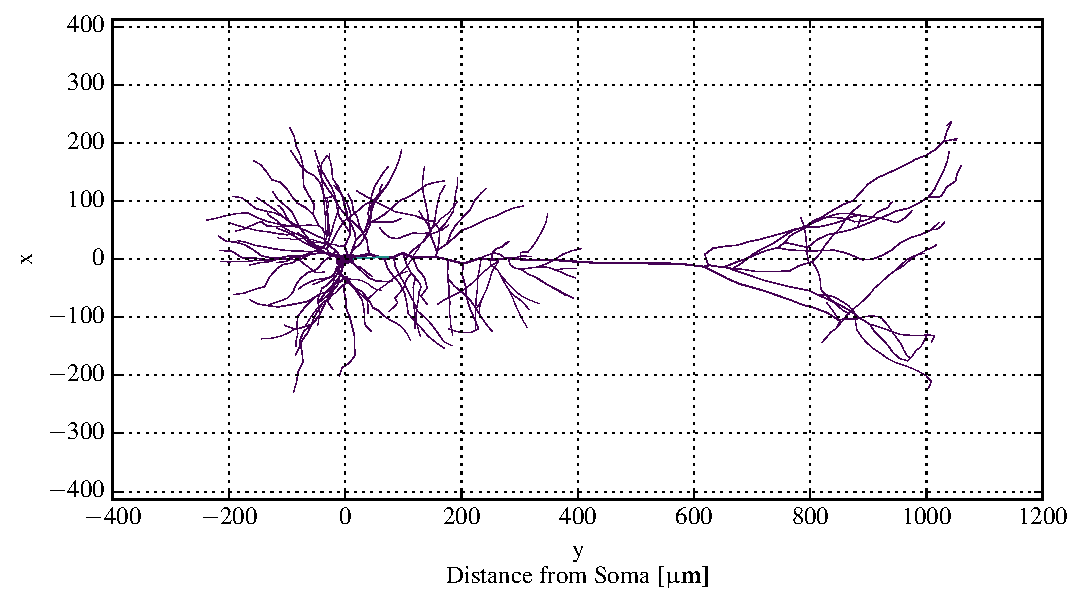
\includegraphics[height=0.4\textheight]{images/ttpc1_morph_xy.pdf}\\
    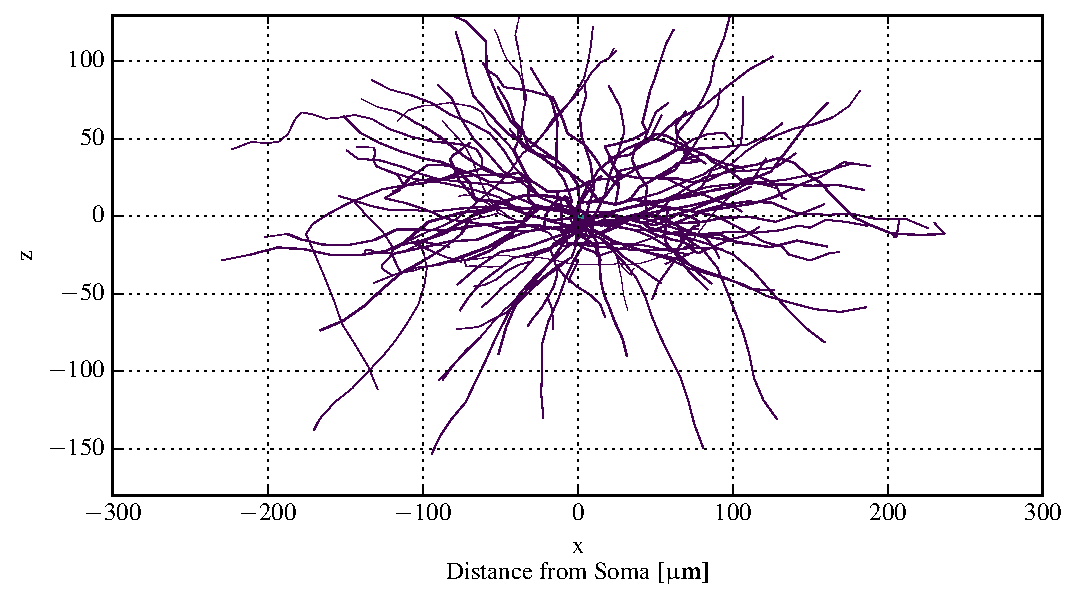
\includegraphics[height=0.4\textheight]{images/ttpc1_morph_xz.pdf}
\end{frame}

\begin{frame}{L5\_MC\_bAC217\_3}{}
    \centering
    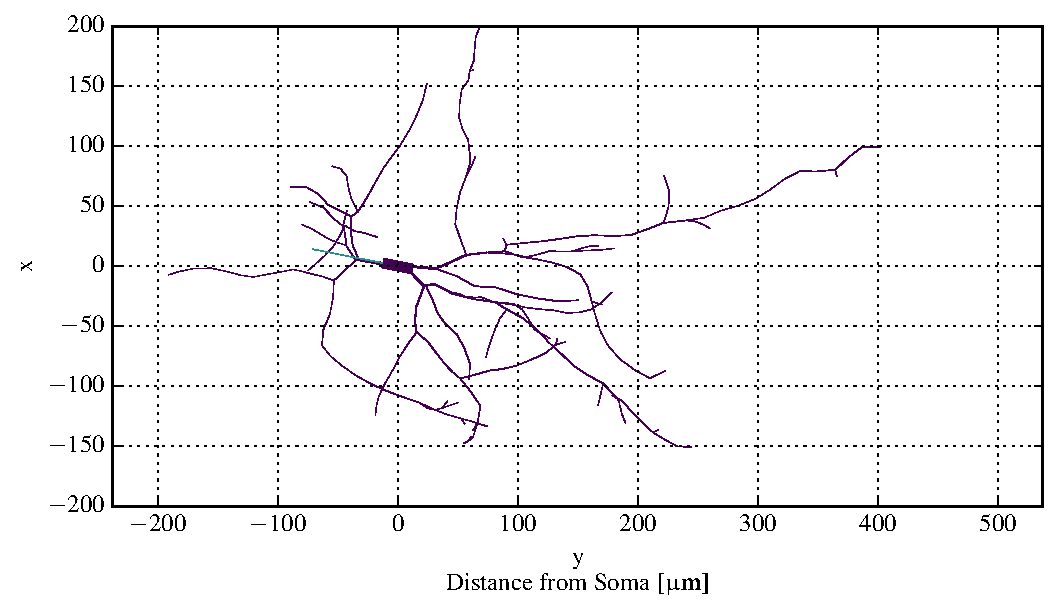
\includegraphics[height=0.4\textheight]{images/mc_morph_xy.pdf}\\
    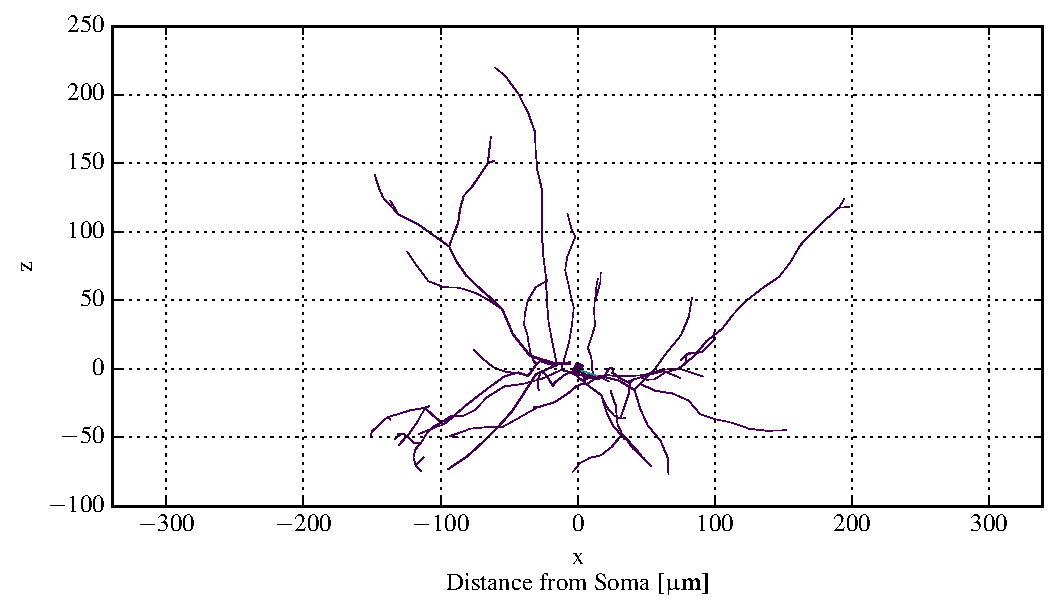
\includegraphics[height=0.4\textheight]{images/mc_morph_xz.pdf}
\end{frame}


\begin{frame}{TTPC1 Spike \SI{20}{\micro\metre}}{}
    \centering
    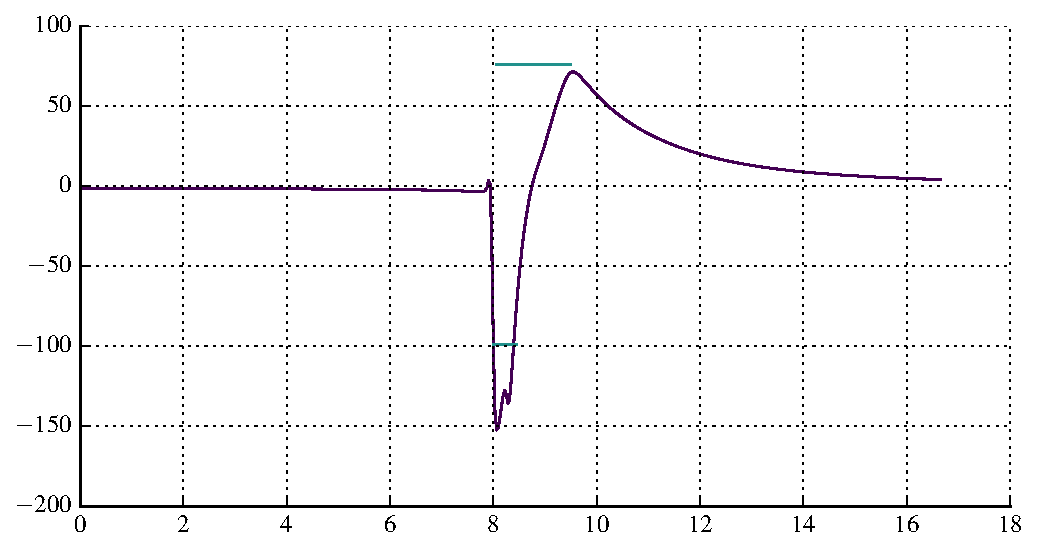
\includegraphics[width=1.0\textwidth]{images/sym_elec_t_170_p_0_n_2.pdf}
\end{frame}

\begin{frame}{TTPC1 Spike \SI{30}{\micro\metre}}{}
    \centering
    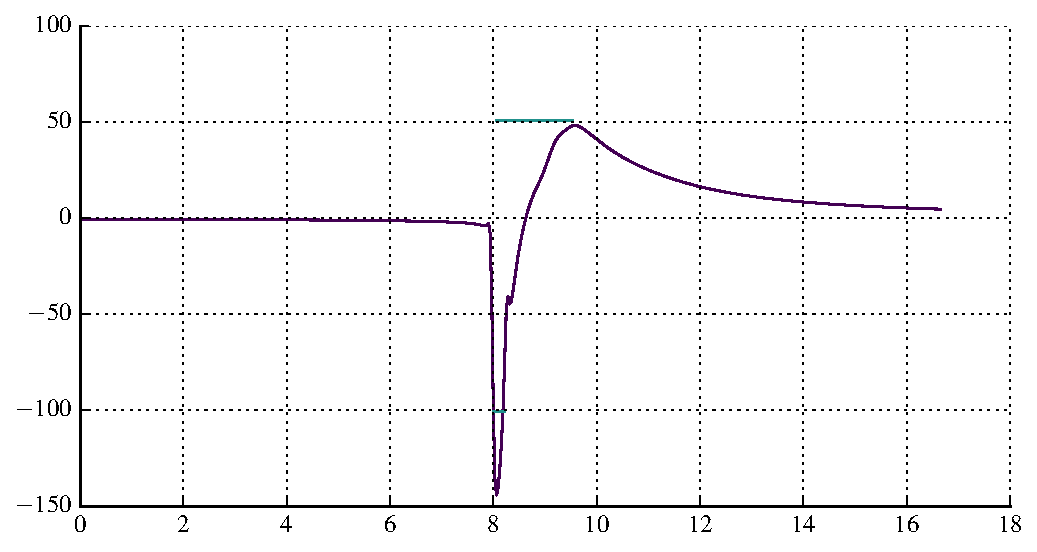
\includegraphics[width=1.0\textwidth]{images/sym_elec_t_170_p_0_n_4.pdf}
\end{frame}

\begin{frame}{TTPC1 Spike \SI{40}{\micro\metre}}{}
    \centering
    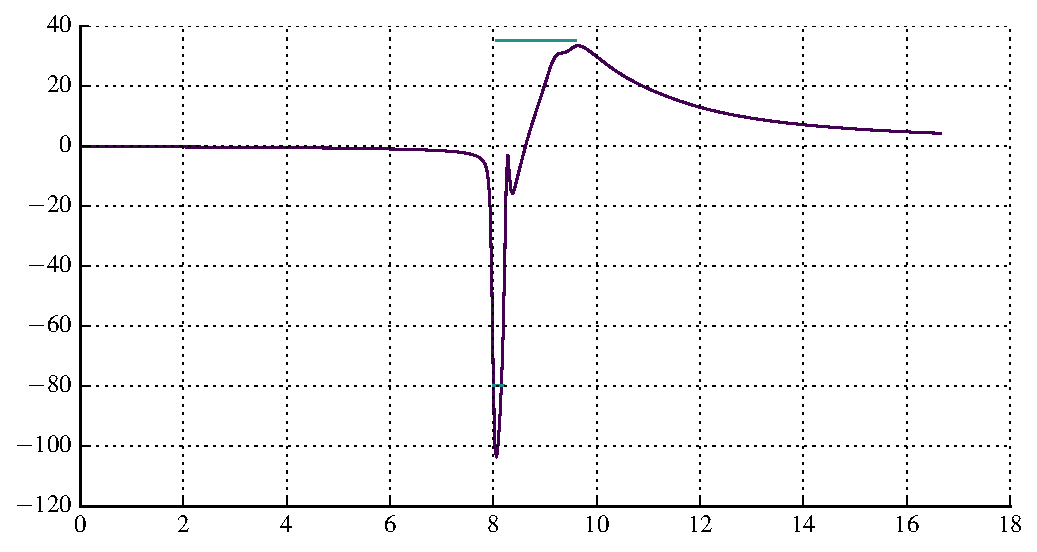
\includegraphics[width=1.0\textwidth]{images/sym_elec_t_170_p_0_n_6.pdf}
\end{frame}

\begin{frame}{TTPC1 Spike \SI{50}{\micro\metre}}{}
    \centering
    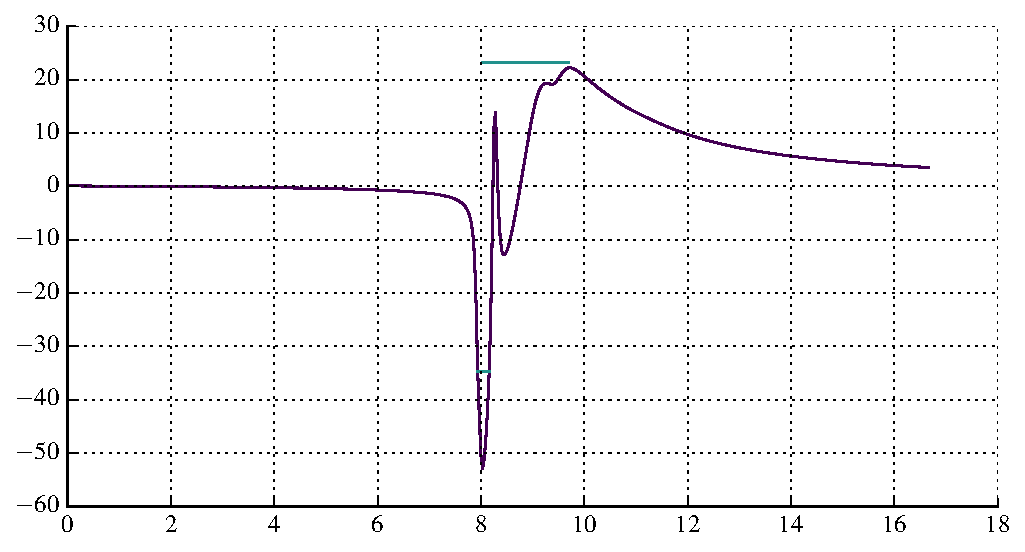
\includegraphics[width=1.0\textwidth]{images/sym_elec_t_170_p_0_n_8.pdf}
\end{frame}

\begin{frame}{TTPC1 Electrodes in Cone Positions}{}
    \centering
    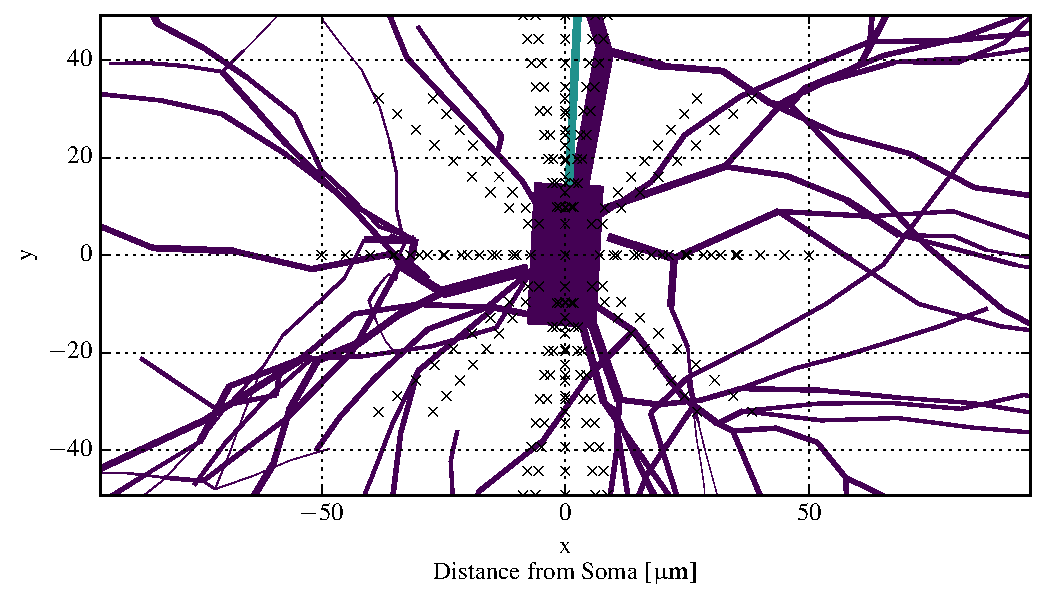
\includegraphics[width=1.0\textwidth]{images/sym_morph_elec.pdf}
\end{frame}

\begin{frame}{TTPC1 Amplitude}{}
    \centering
    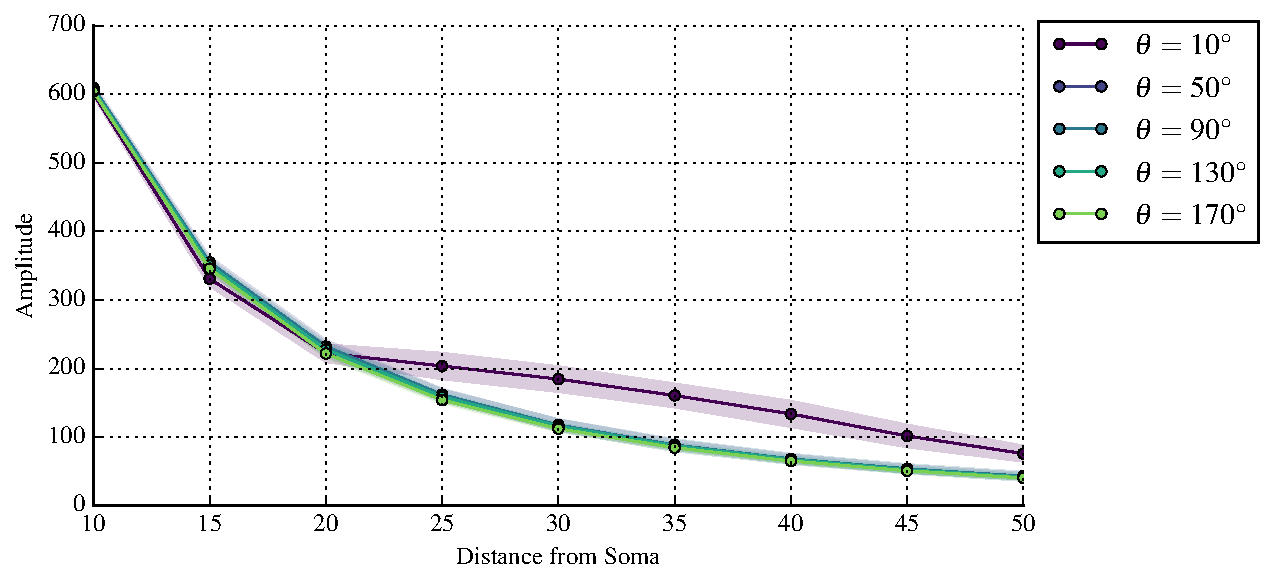
\includegraphics[width=1.0\textwidth]{images/sym_spike_amps_II.pdf}
\end{frame}

\begin{frame}{TTPC1 Spike Width I - peak-to-peak}{}
    \centering
    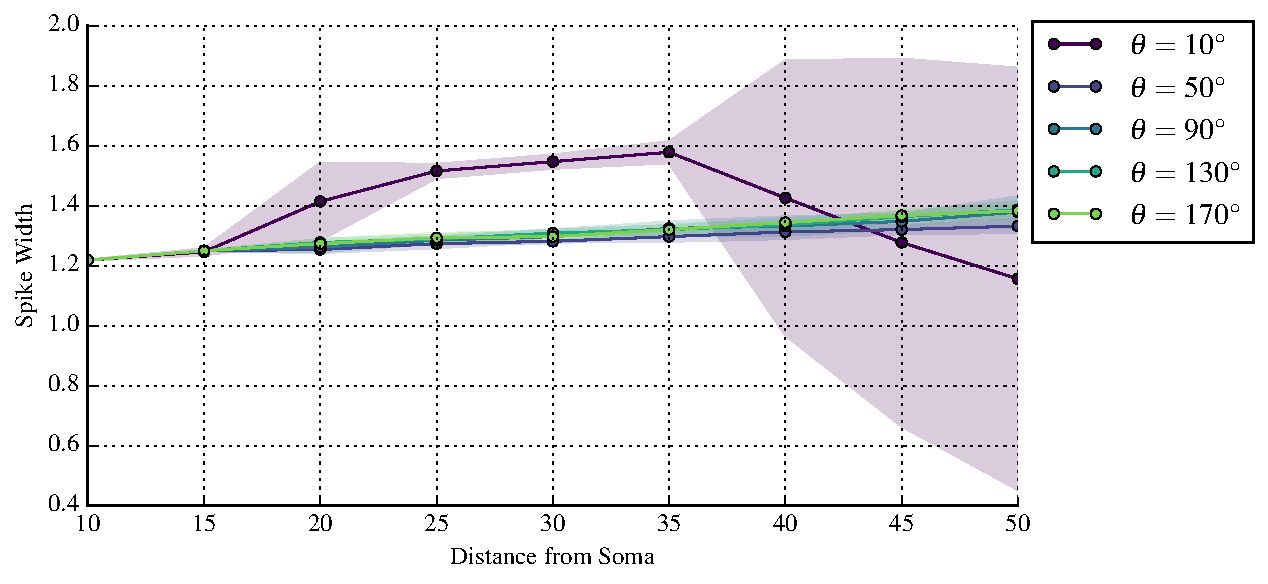
\includegraphics[width=1.0\textwidth]{images/sym_spike_width_I.pdf}
\end{frame}

\begin{frame}{TTPC1 Spike Width II - Half Amplitude}{}
    \centering
    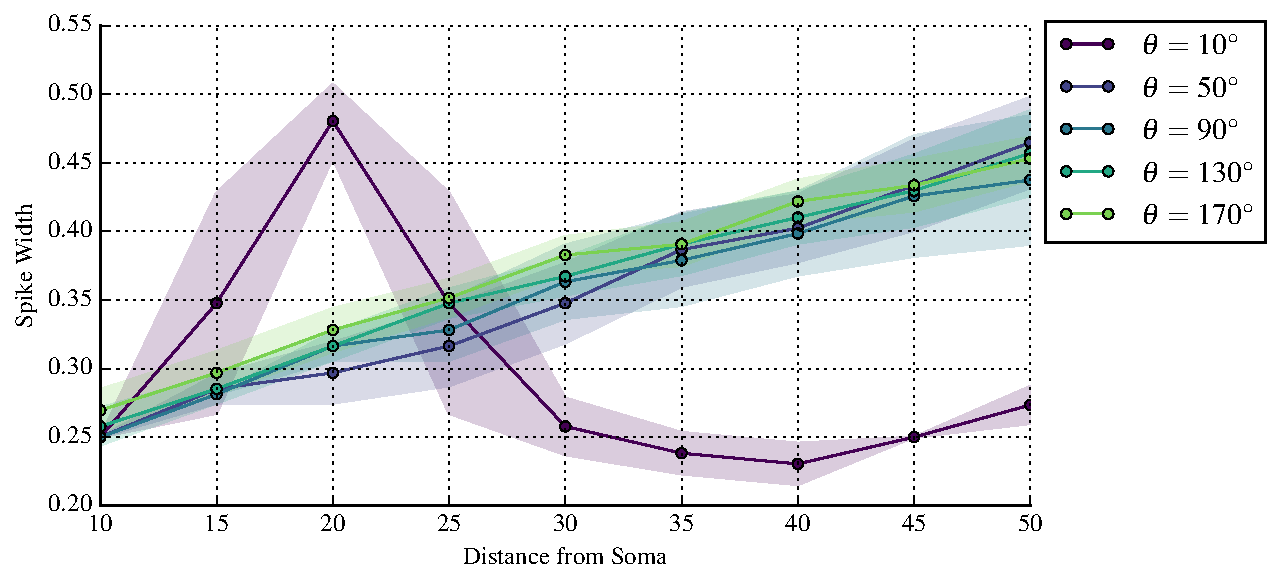
\includegraphics[width=1.0\textwidth]{images/sym_spike_width_II.pdf}
\end{frame}

\begin{frame}{All Neurons Random Electrodes Amplitude}{}
    \centering
    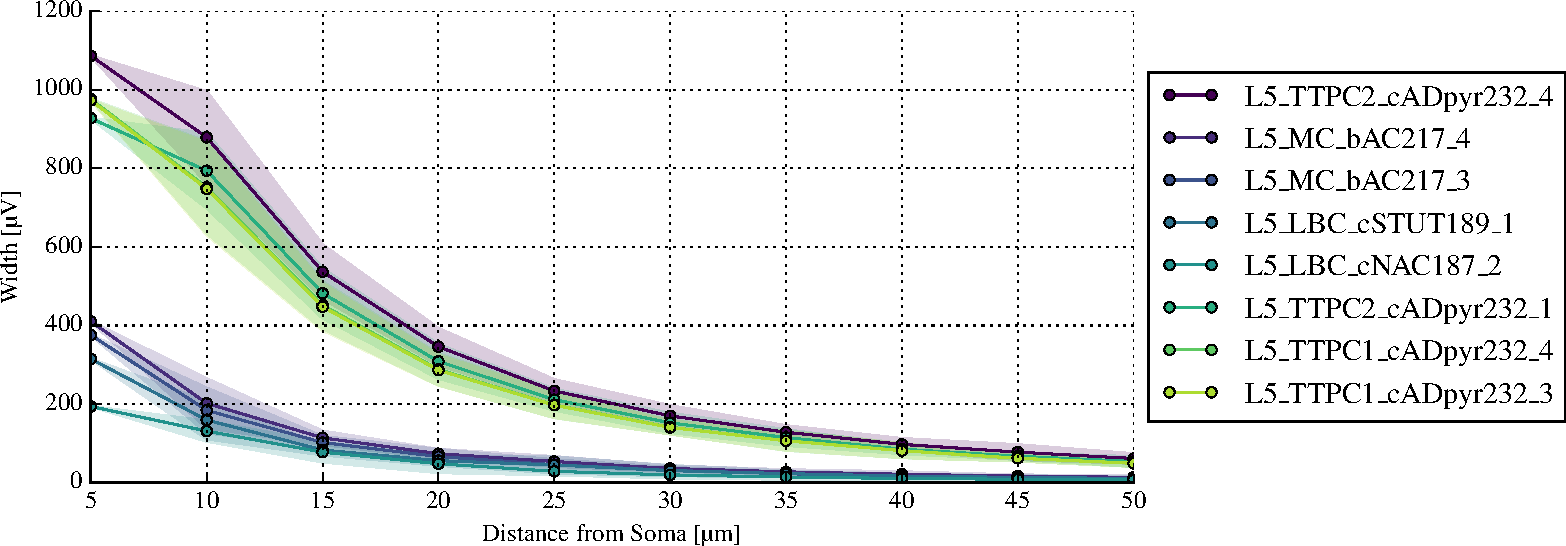
\includegraphics[width=1.0\textwidth]{images/singles_amps_II_all.pdf}
\end{frame}

\begin{frame}{All Neurons Random Electrodes Width I \& II}{}
    \centering
    \begin{figure}
    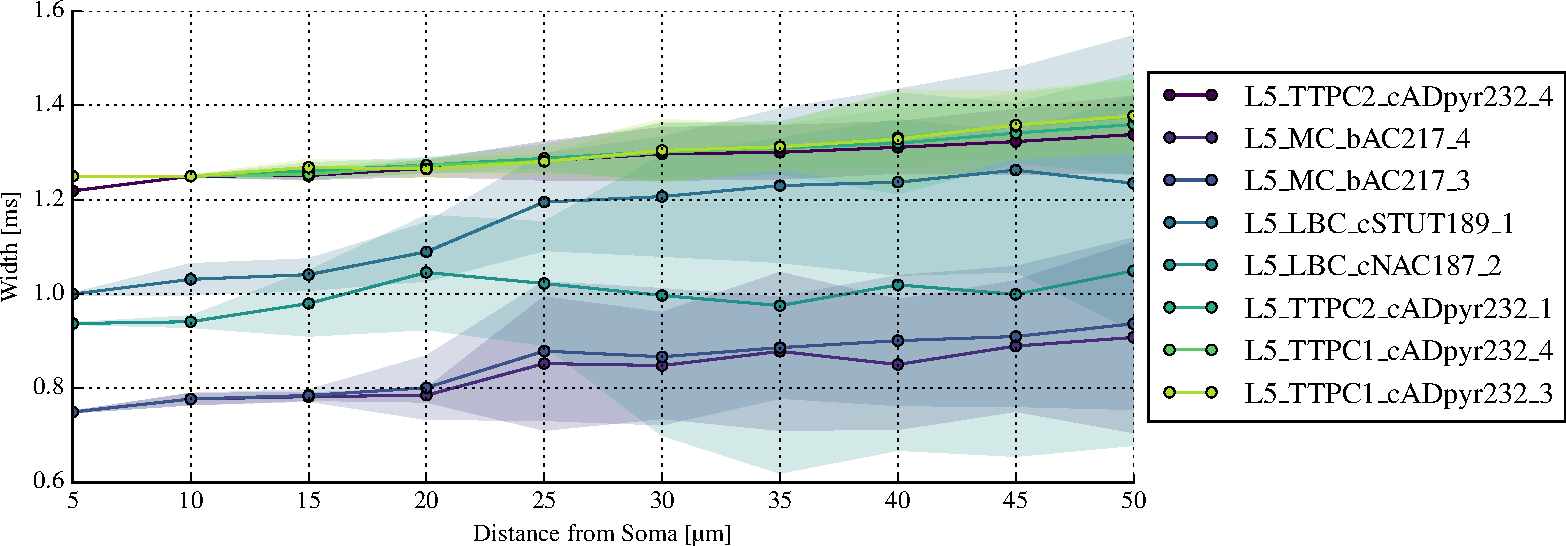
\includegraphics[height=0.4\textheight]{images/singles_widths_I_all.pdf}\\
    \end{figure}
    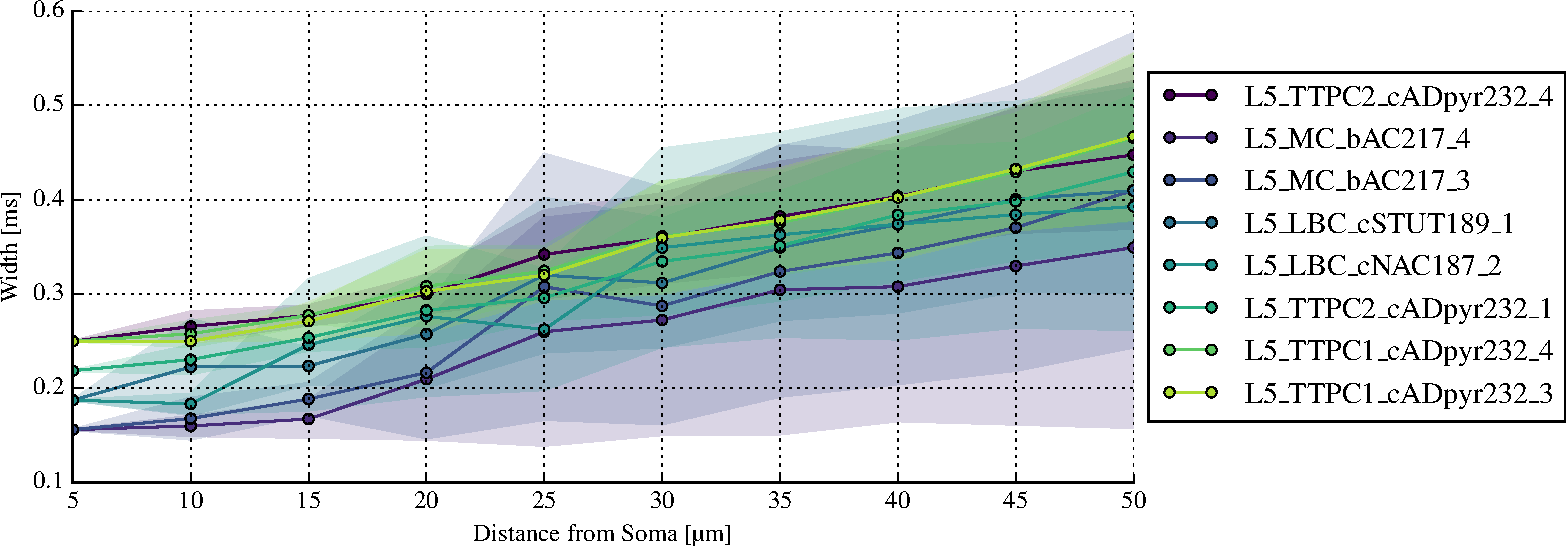
\includegraphics[height=0.4\textheight]{images/singles_widths_II_all.pdf}
\end{frame}

\begin{frame}{All Neurons Random Electrodes Amplitude}{}
    \centering
    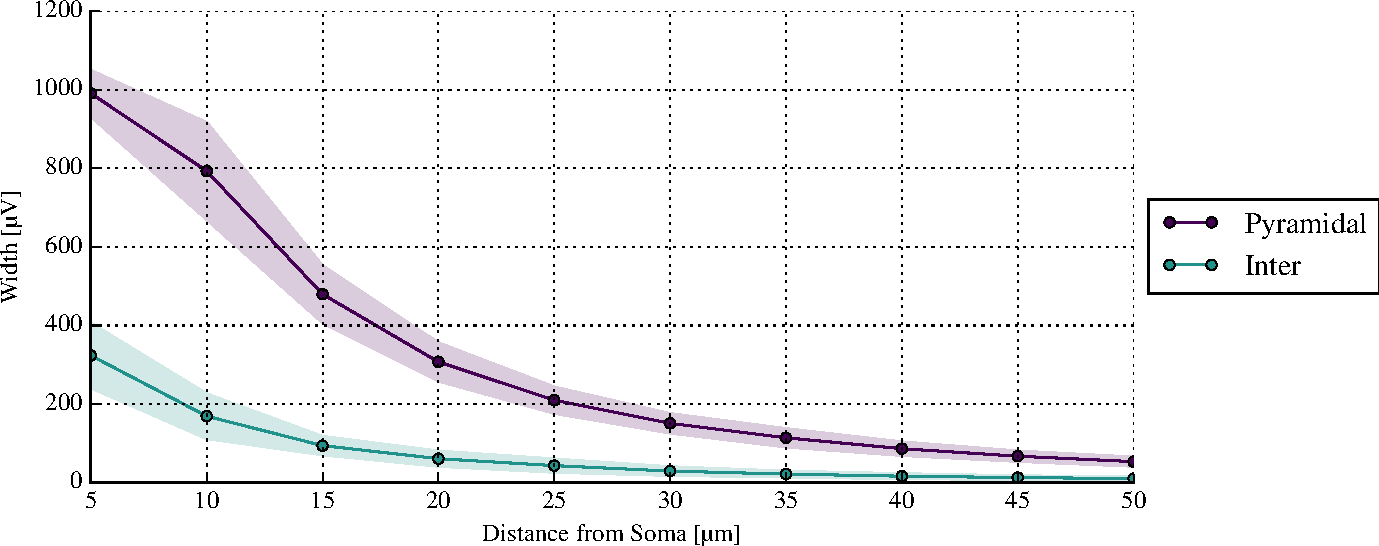
\includegraphics[width=1.0\textwidth]{images/amps_II_all.pdf}
\end{frame}

\begin{frame}{All Neurons Random Electrodes Width I \& II}{}
    \centering
    \begin{figure}
    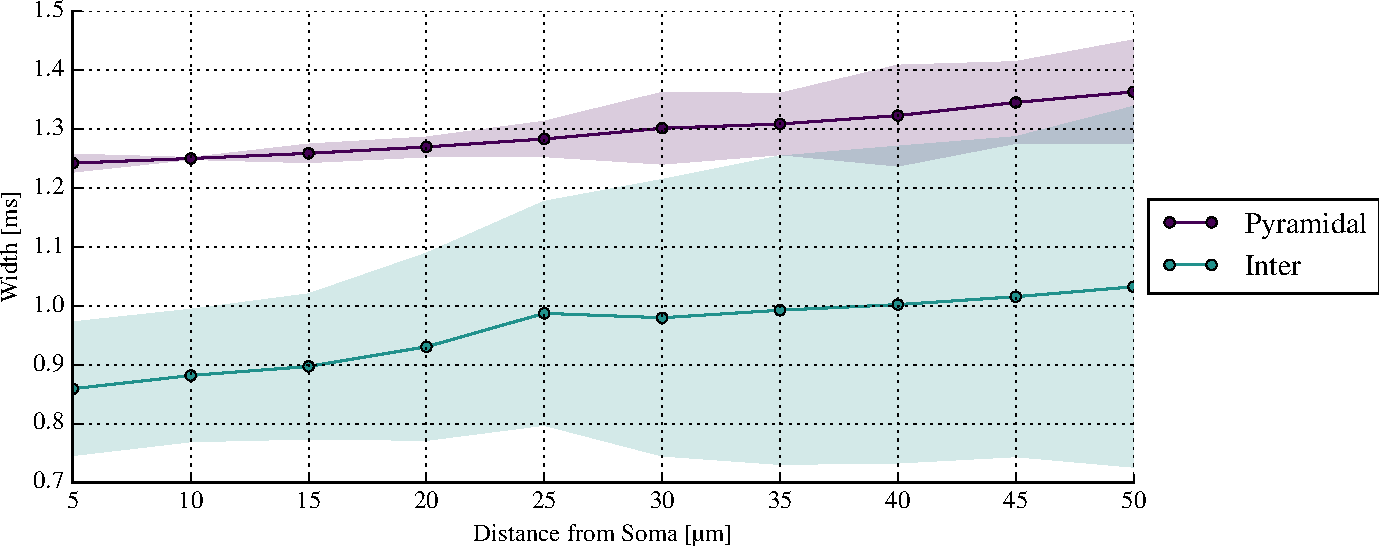
\includegraphics[height=0.4\textheight]{images/widths_I_all.pdf}\\
    \end{figure}
    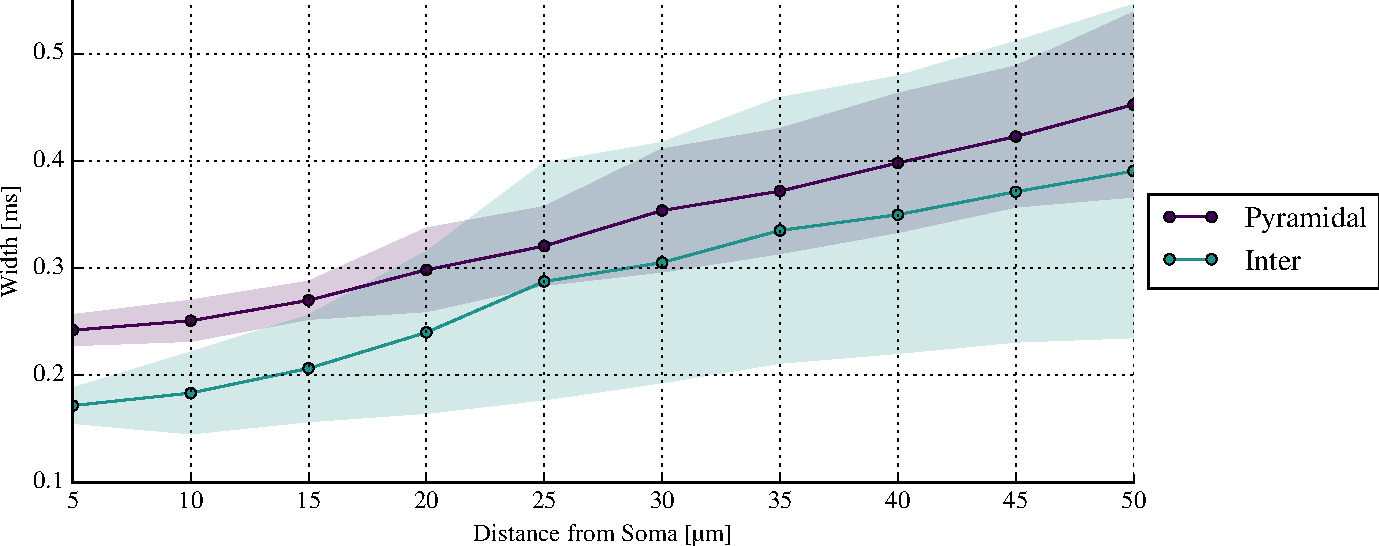
\includegraphics[height=0.4\textheight]{images/widths_II_all.pdf}
\end{frame}

\begin{frame}{All Neurons Random Electrodes Amplitude, Width I \& II}{}
    \centering
    \begin{figure}
    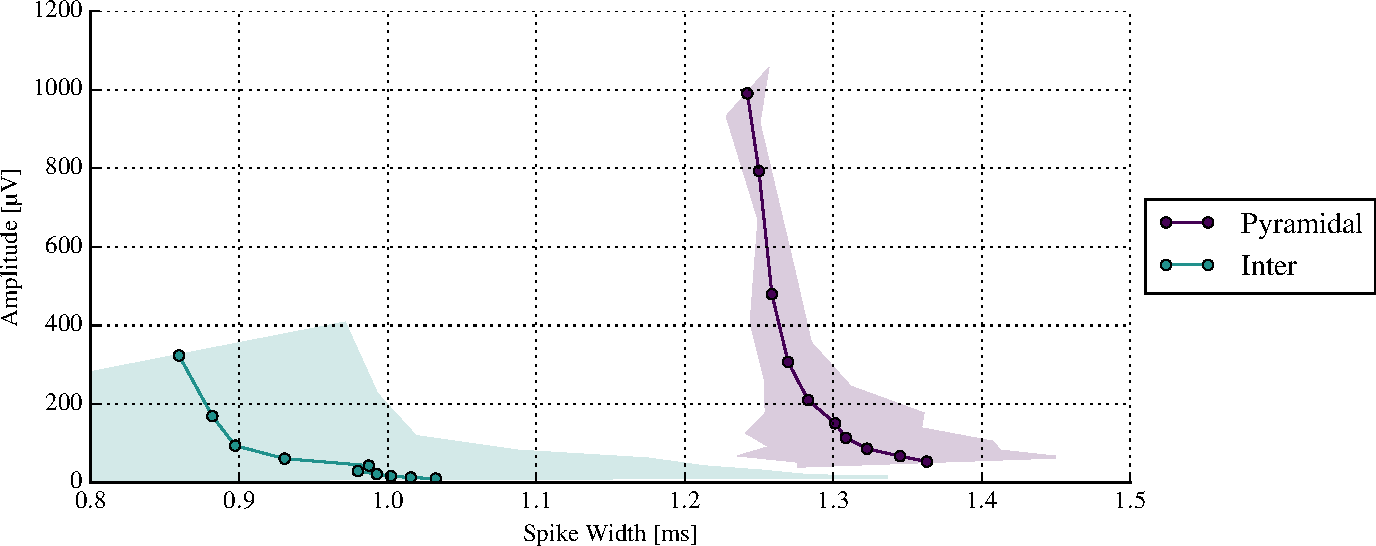
\includegraphics[height=0.4\textheight]{images/amps_widths_I_all.pdf}\\
    \end{figure}
    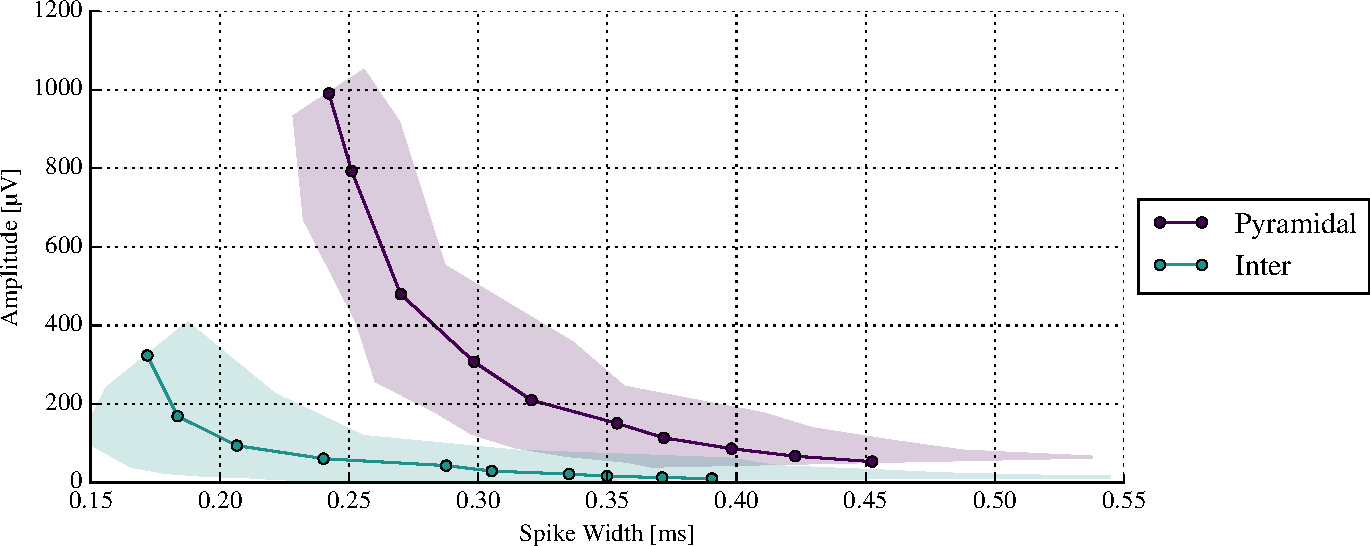
\includegraphics[height=0.4\textheight]{images/amps_widths_II_all.pdf}
\end{frame}

\begin{frame}{Filtered \SI{300}{\hertz} Amplitude, Width I \& II}{}
    \centering
    \begin{figure}
    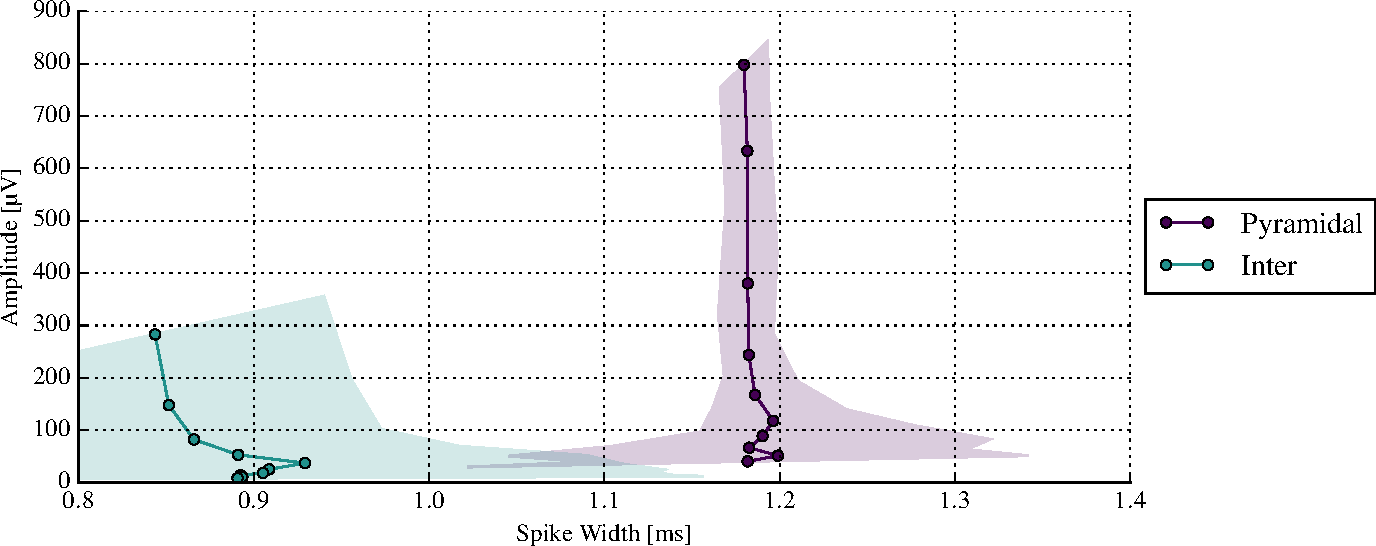
\includegraphics[height=0.4\textheight]{images/filt300_amps_widths_I_all.pdf}\\
    \end{figure}
    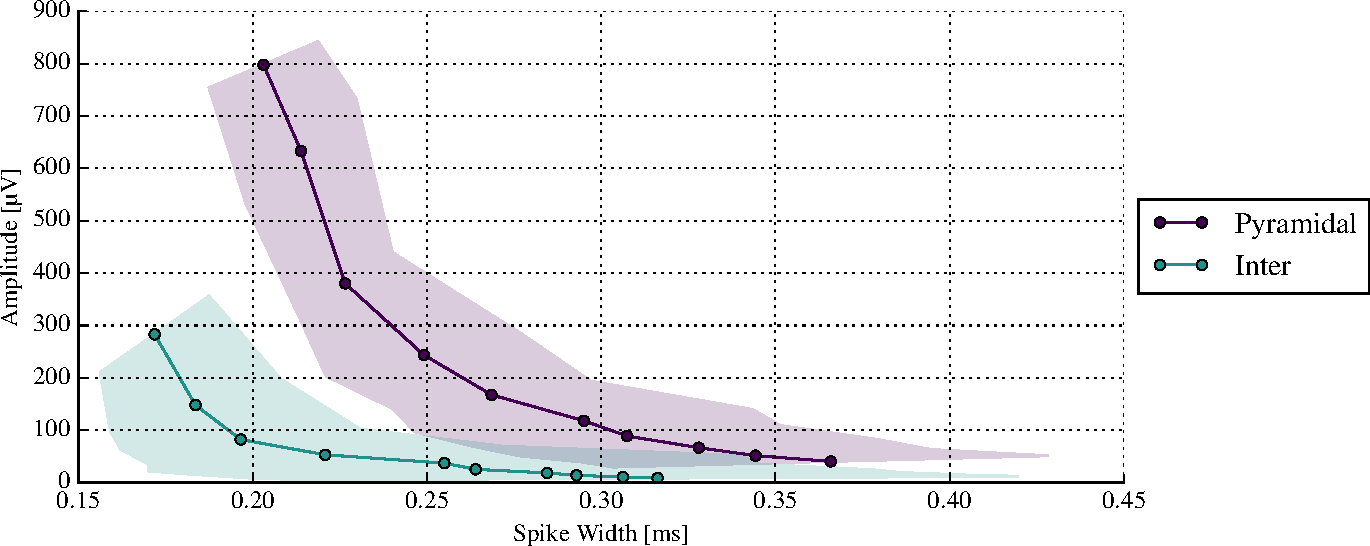
\includegraphics[height=0.4\textheight]{images/filt300_amps_widths_II_all.pdf}
\end{frame}

\begin{frame}{Filtered \SI{800}{\hertz} Amplitude, Width I \& II}{}
    \centering
    \begin{figure}
    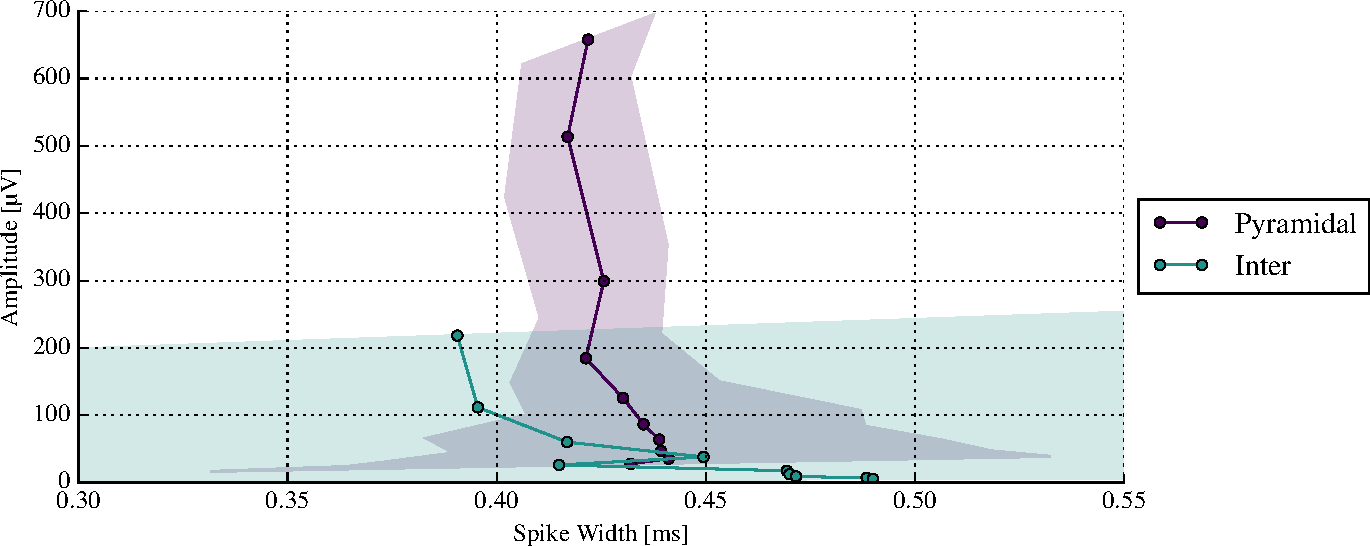
\includegraphics[height=0.4\textheight]{images/filt800_amps_widths_I_all.pdf}\\
    \end{figure}
    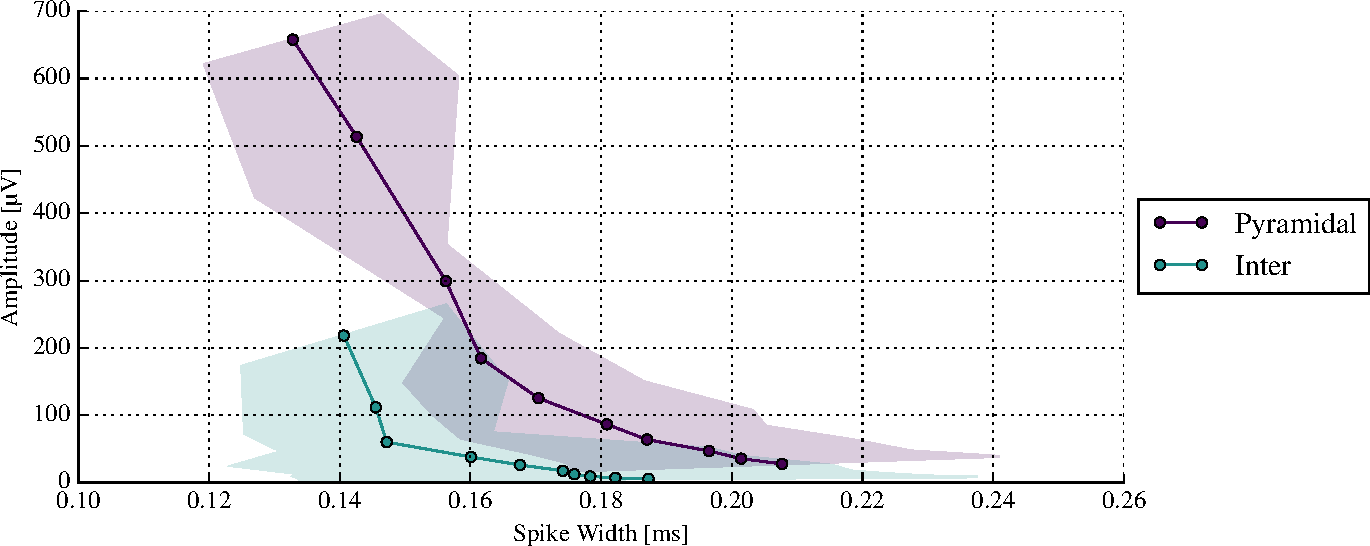
\includegraphics[height=0.4\textheight]{images/filt800_amps_widths_II_all.pdf}
\end{frame}

\begin{frame}{TTPC1 \SI{30}{\micro\metre} from Soma Unfiltered }{}
    \centering
    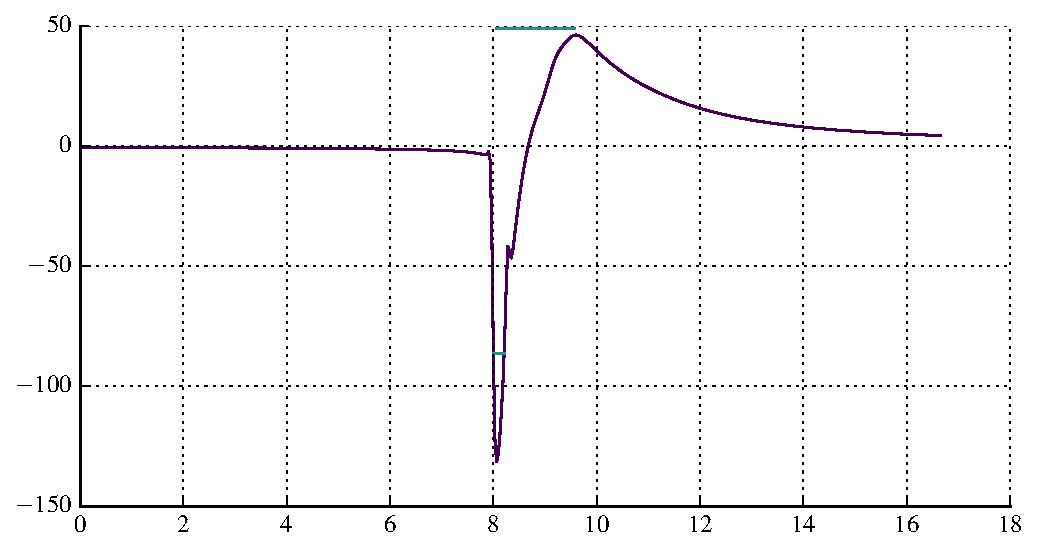
\includegraphics[width=1.0\textwidth]{images/sym_middle_elec_spike.pdf}
\end{frame}

\begin{frame}{TTPC1 \SI{30}{\micro\metre} from Soma \SI{300}{\hertz} }{}
    \centering
    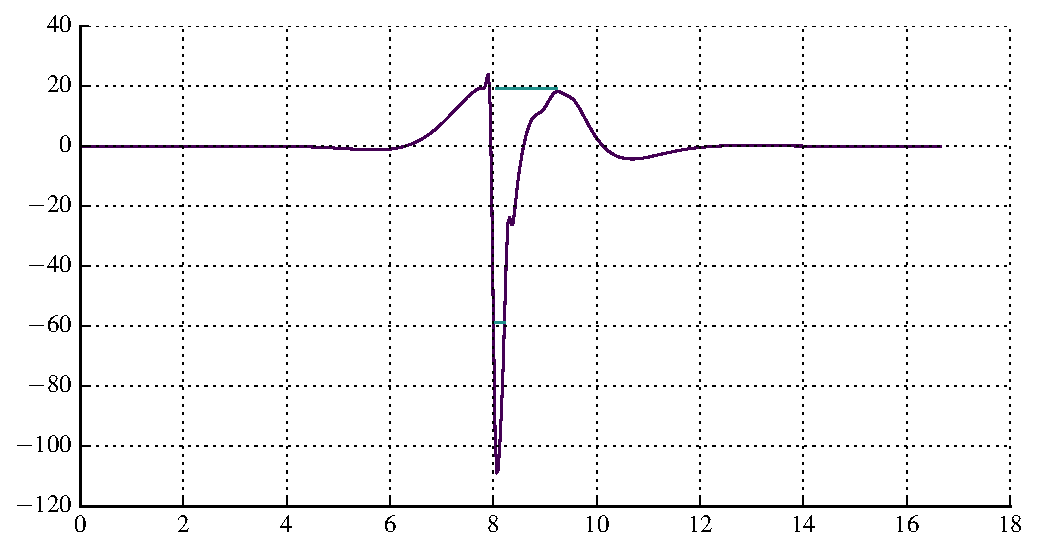
\includegraphics[width=1.0\textwidth]{images/symfilt300_middle_elec_spike.pdf}
\end{frame}

\begin{frame}{TTPC1 \SI{30}{\micro\metre} from Soma \SI{500}{\hertz} }{}
    \centering
    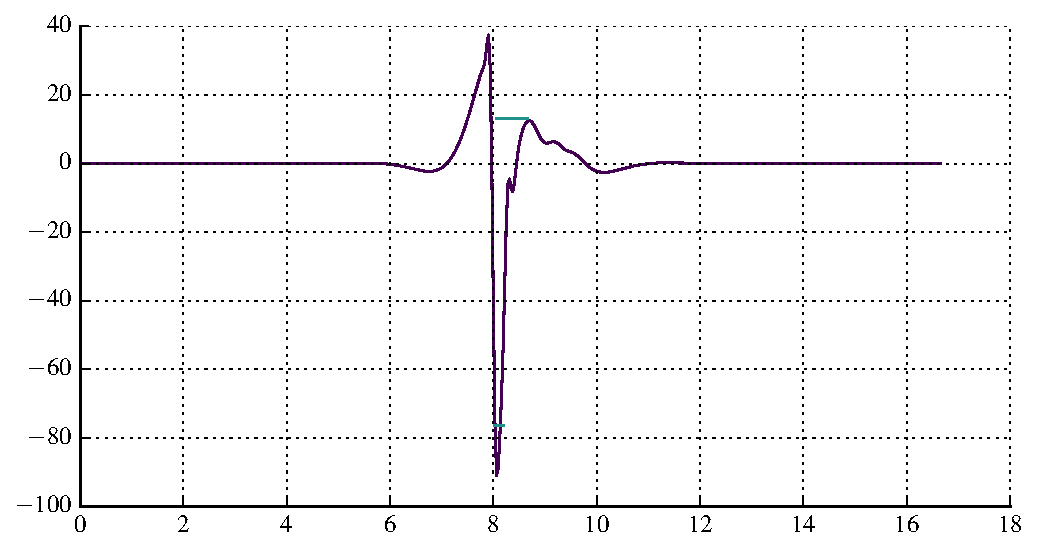
\includegraphics[width=1.0\textwidth]{images/symfilt500_middle_elec_spike.pdf}
\end{frame}

\begin{frame}{TTPC1 \SI{30}{\micro\metre} from Soma \SI{800}{\hertz} }{}
    \centering
    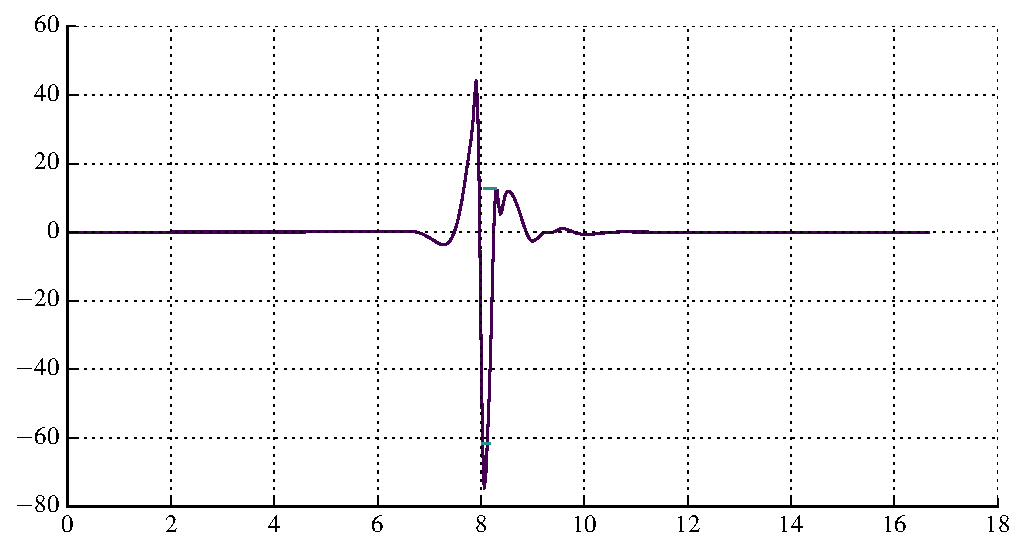
\includegraphics[width=1.0\textwidth]{images/symfilt800_middle_elec_spike.pdf}
\end{frame}

\begin{frame}{TTPC1 Grid Amplitude}{}
    \centering
    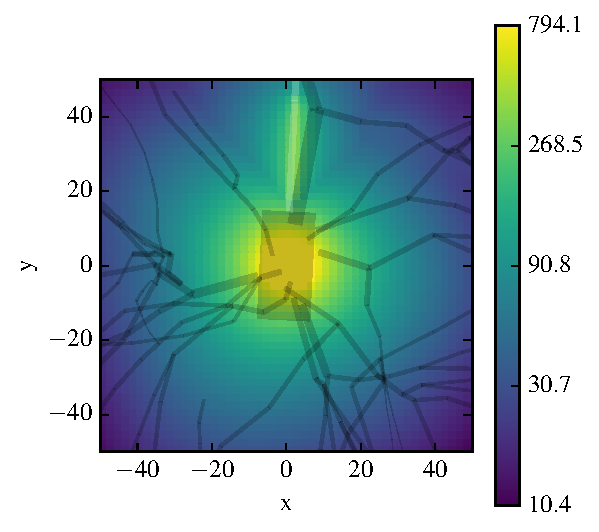
\includegraphics[width=.8\textwidth]{images/ttpc1_grid_dense_gradient.pdf}
\end{frame}

\begin{frame}{TTPC1 Grid Width}{}
    \centering
    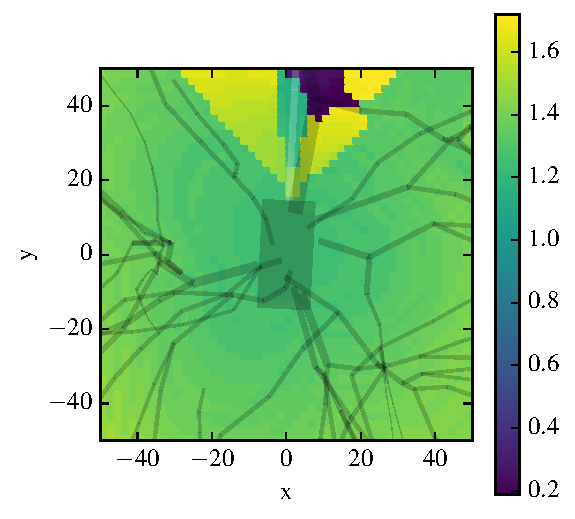
\includegraphics[width=.8\textwidth]{images/ttpc1_grid_dense_width.pdf}
\end{frame}

\begin{frame}{MC Grid Amplitude}{}
    \centering
    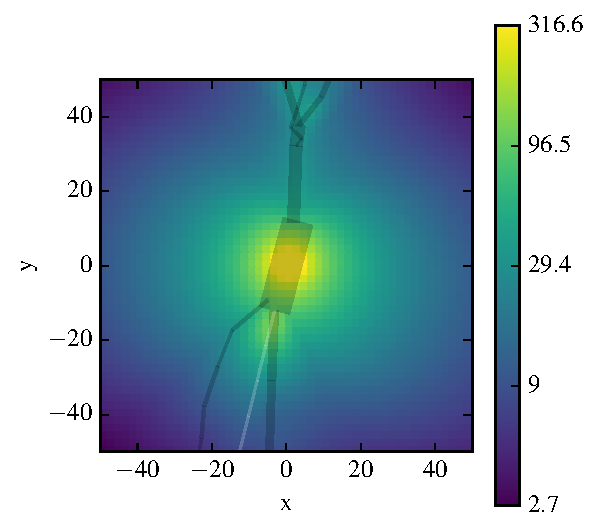
\includegraphics[width=.8\textwidth]{images/grid_dense_gradient.pdf}
\end{frame}

\begin{frame}{MC Grid Width}{}
    \centering
    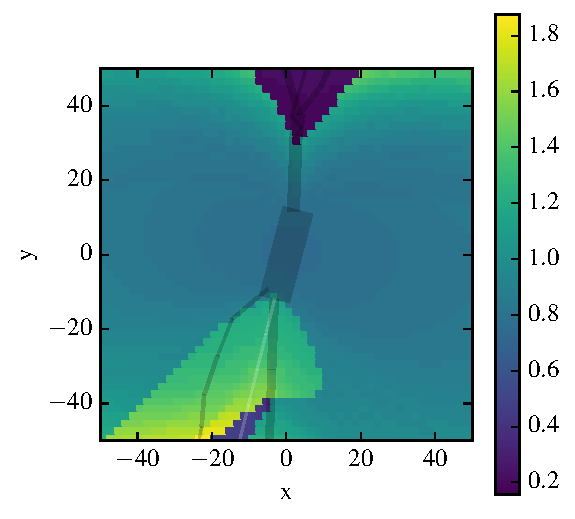
\includegraphics[width=.8\textwidth]{images/grid_dense_width.pdf}
\end{frame}
\end{document}


